\documentclass[a4paper,11pt]{article}
\usepackage[utf8]{inputenc}
\usepackage{amsmath}
\usepackage{amsfonts}
\usepackage{amssymb}
\usepackage{graphicx}

\numberwithin{equation}{section}
\renewcommand\thesubsection{\alph{subsection}}
\newcommand{\bvp}[1]{\mathbf{#1}'}
\newcommand{\bv}[1]{\mathbf{#1}}
\newcommand{\pp}[1]{#1'}


%opening
\title{Thesis Proposal: Separating Cyclostationary Signals using the Nonlinear Dynamics of Continuous-Time Recurrent Networks}
\author{Vince Baker}

\begin{document}

\maketitle

\section{Introduction} 
The human brain hosts advanced cognitive processes that remain only partially understood.
Computational neuroscience seeks to understand brain functions through brain modeling at several levels of physical fidelity.
Computational biophysics provides insight into the lowest levels of neural functions while nonlinear dynamics provides tools for understanding some aspects of cognition.
The liquid state machine (or resevoir computing) computational model uses a nonlinear recurrent network as a resevoir of chaotic dynamics.
Inputs to the resevoir evoke complex states with memory.
Readouts from the resevoir can then be trained to use the resevoir to separate complex temporal inputs.
\\ \\
Resevoir computing has branches in both computational neuroscience (liquid state machines) and machine learning (echo state networks).
The approaches are similar in that they invoke an untrained, high-dimensional resevoir with a trained readout.
The types of networks used are different: echo state networks are typically discrete networks with random sparse connections while liquid state machines are continuous-time networks with biologically inspired connections.
Recently, new echo state network models have been created using a few very fast photonic nodes and space-time coding to mimic a large spatial network.
This work will focus on both approaches to continuous-time networks.
\\ \\
The key research problem will be to separate time series signals using a recurrent continuous-time network. 
Test signals will include sine waves of different frequencies, modulated sine waves, and chaotic signals such as Mackey-Glass.

\section{Background}
Echo state network dynamics include (untrained) input weights $W_{in}$, sparse network weight $W_x$, and trained readout weight $W_{out}$.
The internal network state $x_n$ is driven by both the recurrent connections and the input signal.
The time-dependent output $y_n$ of an echo state network can be defined with the recurrence relation:
\begin{align}
 x_{n+1} &= f(W_x \times x_n + W_{in} \times u_n)\\
 y_n &= W_{out} \times x_n
\end{align}
Where $f()$ is a nonlinear activiation function, typically $\tanh{()} $ (also called a sigmoid activation).
Training of the dense readout layer is accomplished with a simple technique such as linear regression.
\\ \\
Liquid state machinesare described in terms of a continuous filter $L^M$ on a continuous input $u(t)$:
\begin{align}
 x^M(t) &= (L^Mu)(t)\\
 y(t) &= f^M(x^M(t))
\end{align}
The readout map $f^M$ is trained using a biologically plausible mechanism such as the modified perceptron learning rule.

\section{Approach}
Use a recurrent network of nodes with a range of time scales as a near-chaotic resevoir.
Model the networks using apprpriate tools (NEURON, MATLAB ODE, Keras).
Investigate biologically plausible connectivities and determine the onset of the chaotic regime.
Train the readout to recognize cyclostationary signals using a biologically plausible mechanism such as spike-time-dependent plasticity.


\section{Preliminary results}

\section{Work plan}
The approach to the problem includes milestones at every quarter and several decision points.
The first phase (two quarters) is an application of current echo state networks and liquid state machines to signals of interest to identify their strengths and weaknesses and understand the problem space.
The chosen approach is then developed in the second phase (two quarters) through basic simulation.
One quarter is reserved to refine the work into a paper for publication.
The next stage may be an experimental study of nonlinear photonic delay systems OR a high-fidelity simulation using a tool such as NEURON.
One quarter is reserved to refine the experiment or high-fidelity simulation for publication.
The last two quarters are reserved for writing the thesis.
\begin{figure}
 \caption{Schedule}
 \centering
   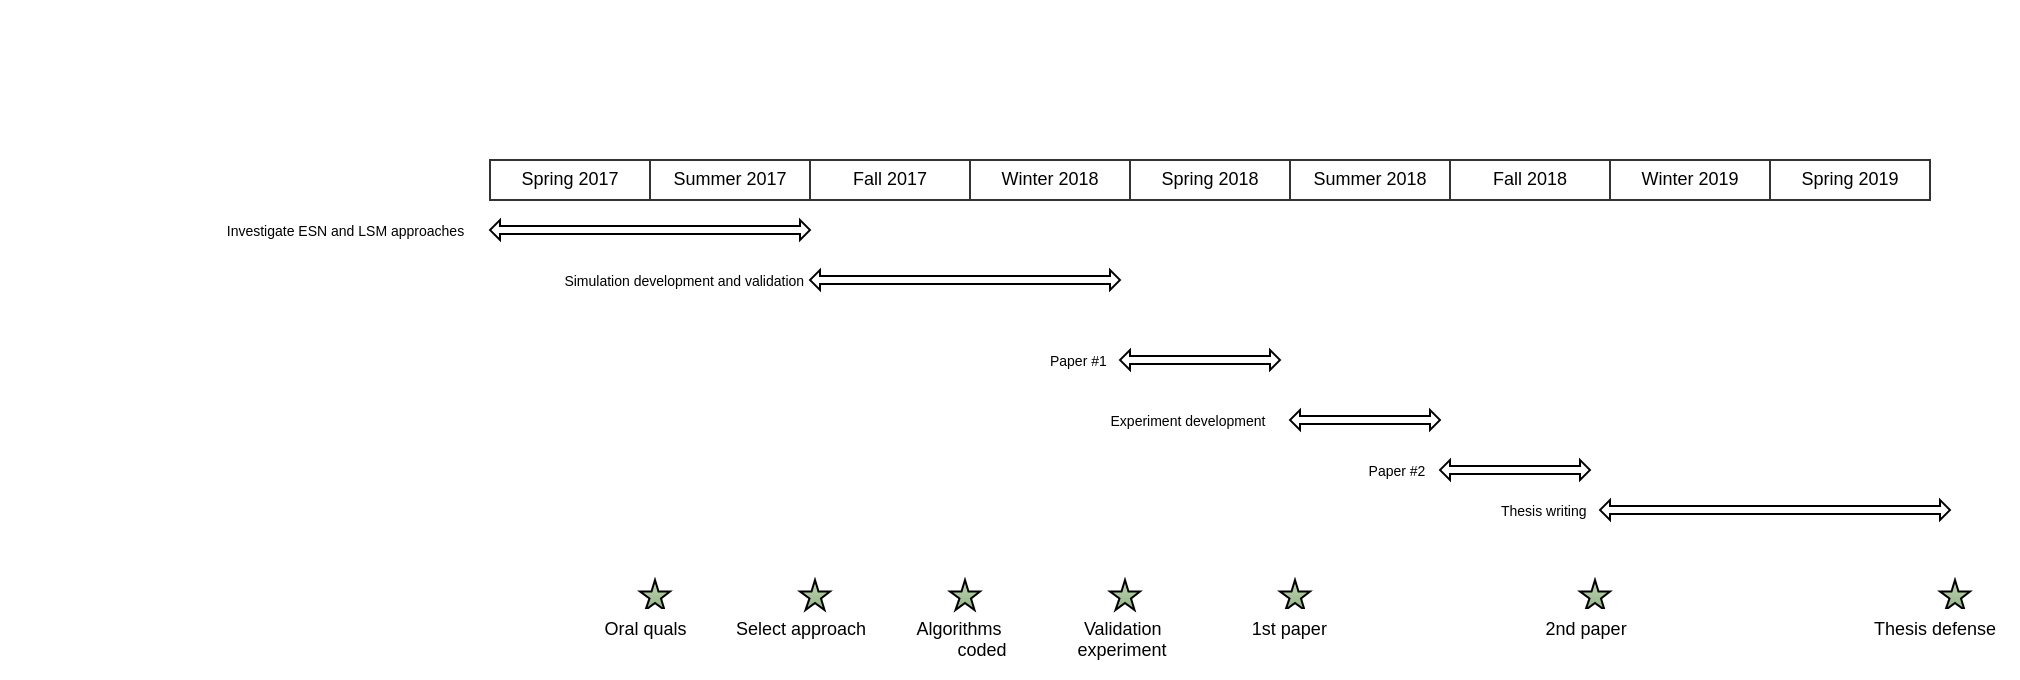
\includegraphics[width=\textwidth]{ThesisSchedule}
\end{figure}

\section{Implications of research}

\section{References}

\end{document}
